\documentclass[a4paper]{article}
% \documentclass[a4paper]{book}

% Imports
\usepackage[utf8]{inputenc}
\usepackage[ngerman]{babel}
\usepackage[T1]{fontenc}
\usepackage{fancyhdr}
\usepackage{epigraph}
\usepackage{subfiles}
\usepackage[acronym,toc]{glossaries}
\usepackage{graphicx}
\usepackage[style=apa]{biblatex}
\usepackage{pdfpages}
\usepackage{hyperref}

\bibliography{../Bibliography}

% Generate the glossary
\makeglossaries

% Title page
\title{Open Source Software \\
    \noindent\rule[0.25ex]{\linewidth}{0.5pt}
    \large Wie nehmen Endanwender Open Source Software wahr?
}

\author{
  Blechschmidt, Til\\
  \texttt{til@blechschmidt.de}\\
  Nordakademie, Elmshorn
  \and
  Peeters, Noah\\
  \texttt{noah.peeters@icloud.com}\\
  Nordakademie, Elmshorn
}

% Numbering
\setcounter{secnumdepth}{3}
\setcounter{tocdepth}{2}

% Quote styling
\setlength\epigraphwidth{.8\textwidth}
\setlength\epigraphrule{0pt}

% Glossery
% \newglossaryentry{oss}{name=OSS, description={Open Source Software}}
\newacronym{oss}{OSS}{Open Source Software}


\begin{document}
    % Title page
    \thispagestyle{fancy}
    \maketitle

    % Abstract
    \begin{abstract}
         \gls{oss} wird in vielen Bereichen eingesetzt. In dieser Arbeit wird analysiert, wie Endanwender \gls{oss} wahrnehmen.
    \end{abstract}
    \newpage

    % TOC
    \tableofcontents
    \clearpage

    % --- Content ---
    \section{Einführung}
        \subsection{Open Source Software}
            \subsubsection{Definition}
                \begin{quote} 
                    \centering 
                    Software wird als Open Source bezeichnet, wenn ihr Quelltext frei zugänglich ist. Sie kann in kommerzieller Software eingesetzt werden, ihre Nutzung muss allerdings nicht kostenfrei sein. 
                \end{quote}
                
        \subsection{Nutzung von Open Source Software}
            Die Nutzung von Open Source Software durch Endanwender kann in zwei Arten unterschieden werden.
            
            \paragraph{Direkte Nutzung}
                Zum einen gibt es die direkte Nutzung, bei der der Nutzer eine Software verwendet, die Open Source ist, also dessen Source Code frei zugänglich ist.
                
                Beispiele für Direkte Nutzung:
                \begin{itemize}
                    \item Wikipedia\footnote{Wikipedia ist eine Konfiguration von Wikimedia, dessen Source Code frei zugänglich ist (\fullcite{wikimedia:download}).}
                    \item Thunderbird\footnote{\fullcite{thunderbird:faq}}
                    \item ... % TODO: mehr Beispiele
                \end{itemize}
                
            \paragraph{Indirekte Nutzung}
                Zum anderen gibt es die indirekte Nutzung. Hier verwendet der Nutzer Software, dessen Source Code nicht frei zugänglich ist, deren Funktionalität aber entscheidend von \gls{oss} Komponenten abhängt. Ohne diese Komponenten wäre die Funktionalität stark eingeschränkt. Hierbei werden folgende Komponenten \textbf{nicht} berücksichtigt:
                
                \begin{itemize}
                    \item Entwicklerwerkzeuge wie Compiler
                    \item Datenbanken wie MySQL
                    \item ... % TODO: gibt es mehr? Apache Web server?
                \end{itemize}
                Der Grund dafür liegt in der Verbreitung dieser Komponenten. % TODO: bessere Erklärung
                
                Beispiele für Indirekte Nutzung:
                \begin{itemize}
                    \item Google Chrome\footnote{\fullcite{chromium:homepage}}
                    \item macOS\footnote{\fullcite{apple:oss}}
                    \item ... % TODO: mehr Beispiele
                \end{itemize}
        
    \section{Umfrage}
        \subsection{Aufbau}
            
        \subsection{Auswertung}
    
    \section{Zusammenfassung}
    
    \clearpage
    \section*{Appendix}
    
        \printglossary[type=\acronymtype]
        \printglossary
        
        \clearpage
        \nocite{*}
        \printbibliography
        
        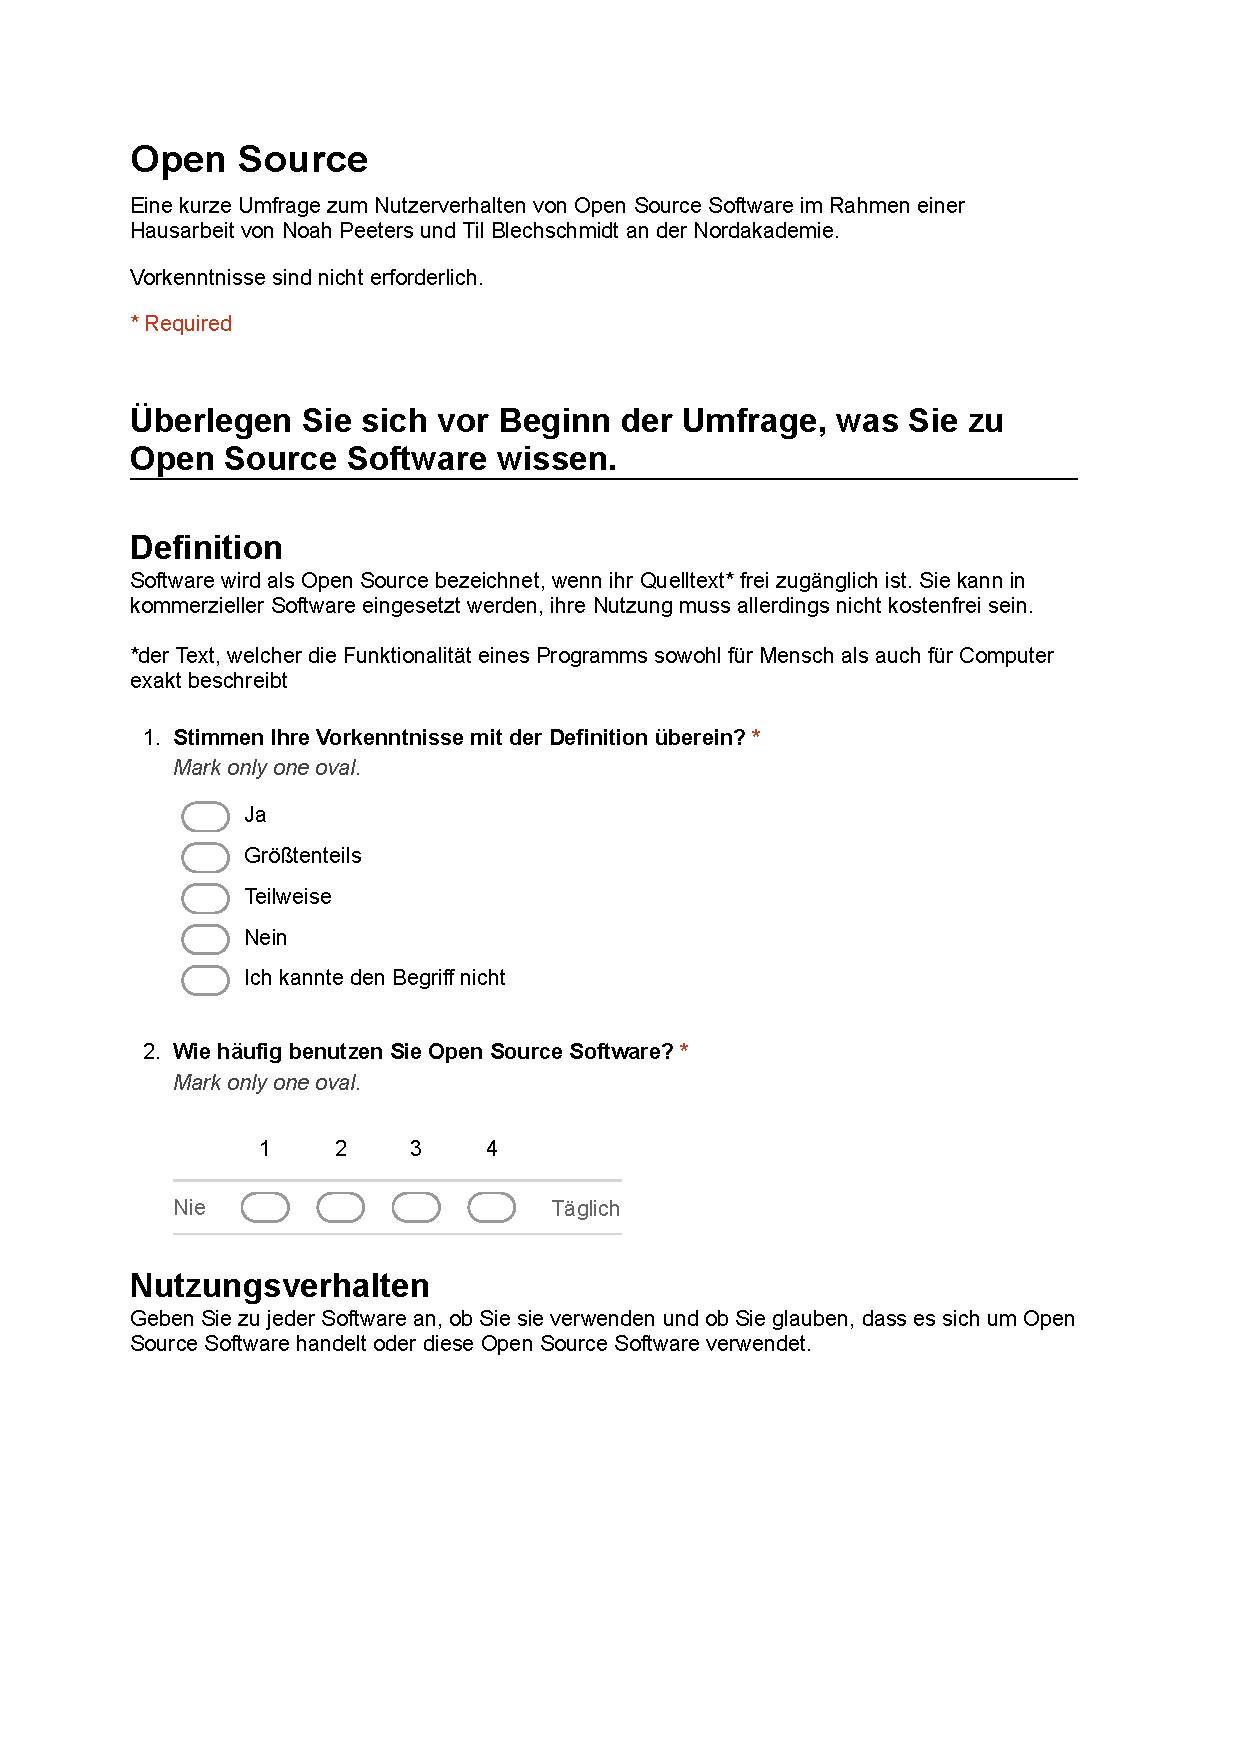
\includepdf[pages={-}]{assets/Umfrage.pdf}

\end{document}
